\documentclass[10pt, letterpaper, titlepage]{article} % Set font here.
% Use 'article' for simple documents; use 'report' for larger documents with chapters;
% use 'book' for even larger documents with parts.
\usepackage[utf8]{inputenc}
\usepackage{geometry}
\usepackage{color,graphicx,overpic} 
\usepackage{fancyhdr} % header/footer stuff
\usepackage{amsmath,amsthm,amsfonts,amssymb}
\usepackage{mathtools} % more math stuff
\usepackage{siunitx} % for SI units, ex. $3.5 ~ \si{kg.s^{-2}}$
\usepackage{hyperref} % for hyperlinks
%\usepackage{apple_emoji}
\usepackage{multicol}
\usepackage{array}
\usepackage{float}
\usepackage{blindtext}
\usepackage{longtable}
\usepackage{scrextend}
\usepackage[font=small,labelfont=bf]{caption}
\usepackage[framemethod=tikz]{mdframed}
\usepackage{calc}
\usepackage{titlesec}
\usepackage{listings}
\usepackage[normalem]{ulem}

\usepackage{listings}
\usepackage{xcolor}

\definecolor{comment}{RGB}{140, 140, 140}
\definecolor{text}{RGB}{204, 204, 204}
\definecolor{string}{rgb}{0.58,0,0}
\definecolor{backcolour}{RGB}{27, 30, 39}
\definecolor{variable}{RGB}{244, 63, 78}

\lstdefinestyle{mystyle}{
    backgroundcolor=\color{backcolour},   
    commentstyle=\color{comment},
    keywordstyle=\color{variable},
    numberstyle=\tiny\color{text},
    stringstyle=\color{string},
    basicstyle=\ttfamily\footnotesize\color{text},
    breakatwhitespace=false,         
    breaklines=true,                 
    captionpos=b,                    
    keepspaces=true,                 
    numbers=left,                    
    numbersep=-10pt,                  
    showspaces=false,                
    showstringspaces=false,
    showtabs=false,                  
    tabsize=4
}

\lstdefinelanguage
   [x64]{Assembler}     % add a "x64" dialect of Assembler
   {morekeywords={	
   }} % etc.
   
\lstdefinelanguage[Motorola68k]{Assembler}{%
	morekeywords={	a0, a1, a2, a3, a4, a5, a6, a7, %
   					d0, d1, d2, d3, d4, d5, d6, d7, %
				   	ABCD,ADD,%
					ADDA,ADDI,ADDQ,ADDX,AND,ANDI,ASL,ASR,BCC,BLS,BCS,BLT,BEQ,BMI,BF,BNE,%
					BGE,BPL,BGT,BT,BHI,BVC,BLE,BVS,BCHG,BCLR,BRA,BSET,BSR,BTST,CHK,CLR,%
					CMP,CMPA,CMPI,CMPM,DBCC,DBLS,DBCS,DBLT,DBEQ,DBMI,DBF,DBNE,DBGE,DBPL,%
					DBGT,DBT,DBHI,DBVC,DBLE,DBVS,DIVS,DIVU,EOR,EORI,EXG,EXT,ILLEGAL,JMP,%
					JSR,LEA,LINK,LSL,LSR,MOVE,MOVEA,MOVEM,MOVEP,MOVEQ,MULS,MULU,NBCD,NEG,%
					NEGX,NOP,NOT,OR,ORI,PEA,RESET,ROL,ROR,ROXL,ROXR,RTE,RTR,RTS,SBCD,%
					SCC,SLS,SCS,SLT,SEQ,SMI,SF,SNE,SGE,SPL,SGT,ST,SHI,SVC,SLE,SVS,STOP,%
					SUB,SUBA,SUBI,SUBQ,SUBX,SWAP,TAS,TRAP,TRAPV,TST,UNLK},%
					sensitive=false,%
					morecomment=[l]*,%
					morecomment=[l] }[keywords,comments,strings]

\lstset{language=[Motorola68k]Assembler}
\lstset{style=mystyle}

\definecolor{mycolor}{rgb}{0, 0, 0}

\pdfinfo{
  /Title (bkongLab4.pdf)
  /Creator (Benjamin Kong)
  /Producer (pdfTeX 1.40.0)
  /Author (Benjamin Kong)
  /Subject (Resume)
  /Keywords (pdflatex, latex,pdftex,tex)}
  

\geometry{top=2.7cm,left=1.8cm,right=1.8cm,bottom=2.7cm}
\setlength{\headheight}{17pt}
\renewcommand{\baselinestretch}{1.5} 
\setlength{\parskip}{0.3cm}
\setlength{\parindent}{0.6cm}
\titlespacing\section{0pt}{12pt plus 4pt minus 2pt}{0pt plus 2pt minus 2pt}

\newcommand{\barrows}{\textcolor{blue}{\Longrightarrow}\quad}
\newcommand{\barrow}{\quad\textcolor{blue}{\Longrightarrow}\quad}  
\newcommand{\sumi}[1][1]{ \sum_{n={#1}}^{\infty} }
\newcommand{\limi}[1][n]{ \lim_{{#1}\to\infty} }

\title{\textbf{\Huge{
\begin{center}
Introduction to\\ Assembly Language\\
\end{center}
}}}
\author{Benjamin Kong | 1573684\\Lora Ma |||| 1570935\\ \\ECE 212 Lab Section H11}

\pagestyle{fancy}
\fancyhf{}
\rhead{Benjamin Kong \& Lora Ma}
\lhead{\textit{Introduction to Assembly Language}}
\rfoot{Page \thepage}

\begin{document} 
\pagenumbering{gobble} 
\maketitle 
\thispagestyle{empty}
\tableofcontents 
\newpage
\pagenumbering{arabic}

\begin{multicols*}{2}

\section{Introduction}
Assembly language is a low-level programming language that is converted to machine code using an assembler. 
Assembly language uses \textit{mnemonics} to represent low-level machine instructions, and this makes it much more readable than machine code.
It is important to note that assembly language is specific to a particular computer architecture and hence may or may not work on different systems.

The purpose of this lab was to become more familiar with assembly language using the NetBurner ColdFire microcontroller board. 
In order to gain experience with assembly language programming, two different programs were created using assembly. 
In the first part of the lab (part A), we created a program that converted an Ascii character to its hexadecimal equivalent. 
For example, `5' is converted to `5' and `B' is converted to `11.'
However, if a character without a hexadecimal equivalent is entered, such as `J,' then an error code results.

For the second part of the lab (part B), we created a program that converts an Ascii letter into its uppercase or lowercase equivalent.
For example, `a' is converted to `A' while `E' is converted to `e.'
If an invalid Ascii character is input (such as an ampersand `\&,' for example), an error code results.


\section{Design}
\subsection{Part A}
First, in our program we initialize address registers $a2$ and $a3$ with addresses and store the number of times the program will loop in a data register. 
Then, we check if at any point in our program the enter key is pressed. 
If it is pressed, the program exits. 
Otherwise, we check if our character is valid through a series of tests. 
First, we check if the given value is less than the hex value `0.'
If it is, then it is an invalid character and the character is replaced with an error code. 
If the value is greater than the hex value `0,' then we compare the value to the hex value `9.'
If the value is greater than `9,' we further test to see if the value is a character between the hex value `A' and the hex value `F.'
If the value is smaller than the hex value `A,' then it is an invalid character. 
If the value is greater than `F', we check if the character is between the hex value `a' and `f.' 
If the value is less than the hex value `a' or greater than the hex value `f,' it is an invalid character. After we've established whether or not the character is valid, we convert the value to its hexadecimal equivalent.

\begin{figure}[H]
   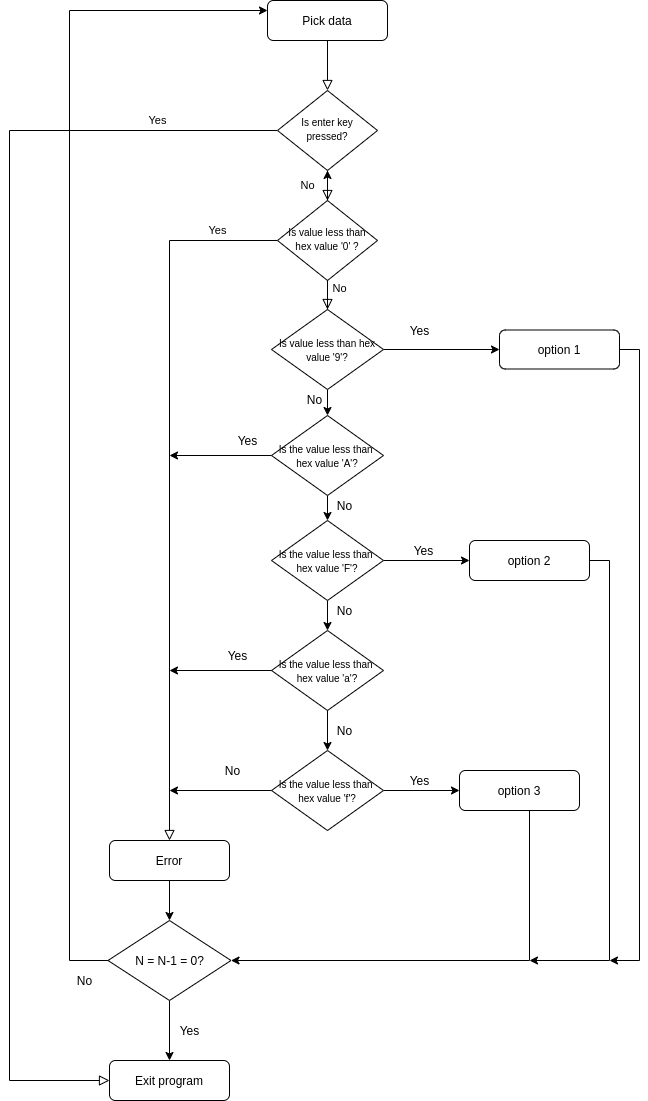
\includegraphics[width=0.38\textwidth]{PartADiagram.png}
   \centering  
   \caption{Flow chart for part A.} 
   \label{figure:1}
\end{figure}

\subsection{Part B}
First, we initialize address registers $a2$ and $a3$ with addresses and store the number of times the program will loop in a data register. 
Then, we check if at any point in our program the enter key is pressed. 
If it is pressed, the program exits. Otherwise, we check if our character is valid through a series of tests. 
First, we check if the character is between the hex value `A' and the hex value `Z.' 
If it is less than `A,' then it is not a valid character. 
If it is greater than `Z,' we further test to see if the character is between the hex value `a' and the hex value `z.' 
If the character is either less than `a' or greater than `z,' it is an invalid character. 
If we have an invalid character, the character is replaced with an error code and we move on to the next value. 
If we have a valid character, we convert the letter to its lowercase/uppercase equivalent.

\begin{figure}[H]
   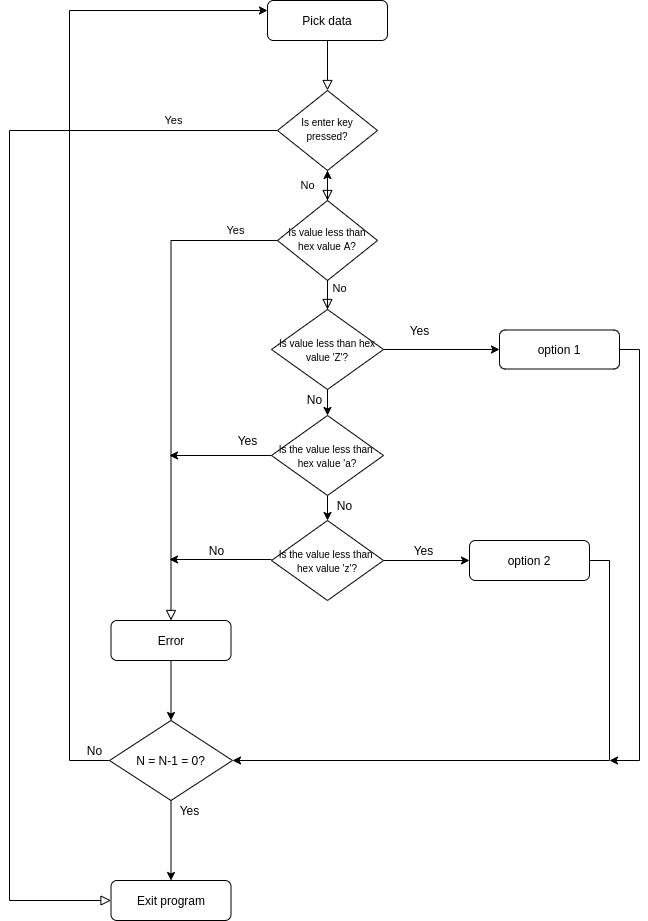
\includegraphics[width=0.38\textwidth]{PartBDiagram.png}
   \centering  
   \caption{Flow chart for part B.} 
   \label{figure:2}
\end{figure}

\section{Testing}
\subsection{Part A}
If properly implemented, part A converts valid Ascii characters that are hexadecimal values into their decimal equivalent. 
In order to test our implementation of part A, we first ran the code with the manual inputs. 
For example, we input various valid and invalid Ascii characters such as `A' (which would be considered valid and should result in an output of `10') and `J' (which would be considered invalid and should result in the error code). 
Once we were confident that our code was working, we moved on to the test cases provided on eClass. 
Upon running these test cases under the supervision of a TA, our program was confirmed to be in working order and we moved on to the next part of the lab, part B.
For a screenshot of the MTTY terminal, please take a look at the appendix.

\subsection{Part B}
If properly implemented, part B converts valid Ascii characters into their lowercase or uppercase counterparts. 
For example, `A' would be converted to `a,' `j' would be converted to `J,' and `\%' would result in an error code since `\%' doesn't have an uppercase or lowercase equivalent. 
After finishing our code for part B, we again tested manual inputs to check that our program functioned as expected.
Once we were confident that our implementation was correct, we moved on to the test cases provided on eClass.
Using these test cases, a TA confirmed that our code functioned correctly and we cleaned up our workstation.
For a screenshot of the MTTY terminal, please take a look at the appendix.


\section{Questions}
\textbf{Q1).} \textit{What happens when there is no exit code `0x0D' provided in the initialization process? Would it cause a problem? Why or why not?}

This would not be an issue since input is limited to 100 inputs. 
This is because the program decrements the value stored at data register $d7$ each time a character is input and the program can only loop if the value at $d7$ is not zero. 
As soon as 100 inputs are present and processed, the value of $d7$ will be zero and the program will exit.

\textbf{Q2).} \textit{How can our code be modified to provide a variable address range? For example, what if I only wanted to convert the first 10 data entries?}

We could initialize another variable representing the address range, say 10, at $d6$. 
For example, we could add the line
\begin{lstlisting}
	move.l #10, %d6
\end{lstlisting}
at the beginning and decrement this each time a data entry is converted. 
If the value at $d6$ is zero, then we stop converting data entries.

\section{Conclusion}
The purpose of this lab was to become more familiar with assembly language using the NetBurner Coldfire microcontroller board.  
In order to do this, we completed two parts: part A, which involved converting valid Ascii characters into the equivalent hexadecimal value; and part B, which involved converting valid uppercase Ascii characters into their lowercase equivalent and vice versa for valid lowercase Ascii characters.

Overall, the lab was a success: both parts of the lab were completed in a timely fashion and our understanding of assembly language was increased. 
Both part A and part B of the lab were shown to work with the test cases provided on eClass.
In the future, we would like to become even more proficient with assembly language and we look forwards to completing future labs. :)

\end{multicols*}

\newpage

\section{Appendix}
\subsection{Part A MTTY Screenshots}
\begin{figure}[H]
   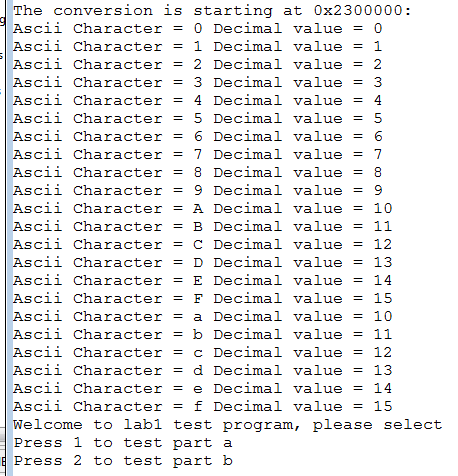
\includegraphics[width=0.38\textwidth]{PartA_1.png}
   \centering  
   \caption{Screenshot of MTTY output for part A using DataStorage.s.} 
   \label{figure:3}
\end{figure}

\begin{figure}[H]
   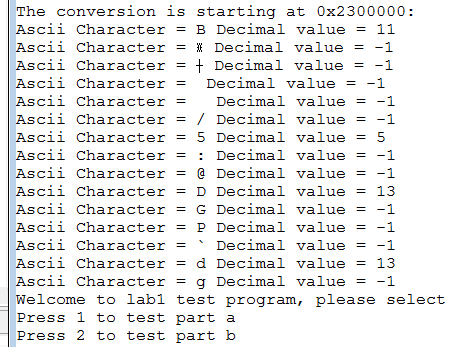
\includegraphics[width=0.38\textwidth]{PartA_2.png}
   \centering  
   \caption{Screenshot of MTTY output for part A using DataStorage1.s.} 
   \label{figure:4}
\end{figure}

\subsection{Part B MTTY Screenshots}
\begin{figure}[H]
   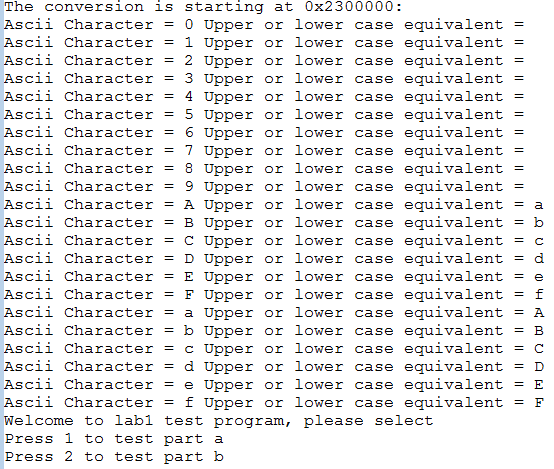
\includegraphics[width=0.38\textwidth]{PartB_1.png}
   \centering  
   \caption{Screenshot of MTTY output for part B using DataStorage.s.} 
   \label{figure:5}
\end{figure}

\begin{figure}[H]
   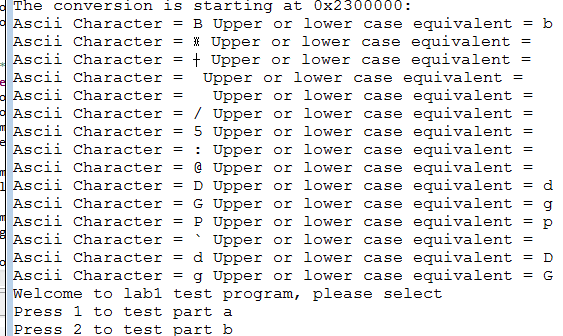
\includegraphics[width=0.38\textwidth]{PartB_2.png}
   \centering  
   \caption{Screenshot of MTTY output for part B using DataStorage1.s.} 
   \label{figure:6}
\end{figure}

\subsection{Part A Assembler Code}
\begin{lstlisting}
	/* DO NOT MODIFY THIS --------------------------------------------*/
	.text
	
	.global AssemblyProgram
	
	AssemblyProgram:
	lea      -40(%a7),%a7 /*Backing up data and address registers */
	movem.l %d2-%d7/%a2-%a5,(%a7)
	/*----------------------------------------------------------------*/
	
	/******************************************************************/
	/* General Information ********************************************/
	/* File Name: Lab1a.s *********************************************/
	/* Names of Students: Lora Ma and Benjamin Kong                  **/
	/* Date: 3 February 2020                                         **/
	/* General Description: Converts Ascii characters to its         **/
	/*                      hex/dec equivalent.                      **/
	/******************************************************************/
	
	move.l #0x43000000, %a2      /* address of values to convert */
	move.l #0x43100000, %a3      /* adresss of converted values to be stored */
	move.l #100, %d7             /* amount of iterations for loop */
	
	
	/* repeat: main loop. Checks each input and converts if possible. */
	repeat:
	move.l (%a2), %d2            /* move value from address into data register */
	move.l %d2, (%a3)            /* move value in data register into address */
	cmpi.l #0x0d, %d2            /* enter key pressed => exit */
	beq done                     /* exits if enter key was pressed */
	
	cmpi.l #0x30, %d2            /* compares the value to hex '0' */
	blt error                    /* not a valid character if less than 0 */
	cmpi.l #0x39, %d2            /* compare the value to hex '9' */
	bgt higher                   /* go to higher to keep testing */
	
	move.l #0x30, %d2            /* move value into data register */
	sub.l %d2, (%a3)             /* subtract data register value from address value */
	bra check                    /* check if done iterating */
	
	
	/* higher: checks if it's a uppercase ascii character */
	higher:
	cmpi.l #0x41, %d2            /* compare value to hex 'A' */
	blt error                    /* not a valid character; go to error */
	cmpi.l #0x46, %d2            /* compare the value to hex 'F' */
	bgt lower                    /* go to lower to keep testing */
	  
	move.l #0x37, %d2            /* move value into data register */
	sub.l %d2, (%a3)             /* subtract value from d2 to value in address */
	bra check                    /* go to check */
	
	
	/* lower: checks if it's a lowercase ascii character */
	lower:
	cmpi.l #0x61, %d2            /* compare the value to hex 'a' */
	blt error                    /* not a valid character; go to error */
	cmpi.l #0x66, %d2            /* compare the value to hex 'f' */
	bgt error                    /* go to continue to keep testing */
	move.l #0x57, %d2            /* move value to data register */
	sub.l %d2, (%a3)             /* subtract d2 from value in address */
	bra check                    /* go to check */
	
	
	/* check: checks if done iterating */
	check:
	add.l #4, %a2                /* increment address by one long word */
	add.l #4, %a3                /* increment address by one long word */
	sub.l #1, %d7                /* subtract 1 from data register */
	cmp.l #0, %d7                /* see if 100 iterations are done */
	beq done                     /* if yes, exit loop and go to done */
	bra repeat                   /* else repeat loop */
	
	
	/* error: moves error code to memory location */
	error:
	move.l #0xFFFFFFFF, (%a3)    /* move error code into memory location */
	add.l #4, %a2                /* increment address by one long word */
	add.l #4, %a3                /* increment address by one long word */
	sub.l #1, %d7                /* subtract value from data register */
	cmp.l #0, %d7                /* compare value with data register*/
	beq done                     /* if equal, exit loop and go to done */
	bra repeat                   /* else repeat loop */
	
	
	/* done: exit point of program */
	done:
	
	
	/*End of program **************************************************/
	
	/* DO NOT MODIFY THIS --------------------------------------------*/
	movem.l (%a7),%d2-%d7/%a2-%a5 /*Restore data and address registers */
	lea      40(%a7),%a7 
	rts
	/*----------------------------------------------------------------*/
\end{lstlisting}

\subsection{Part B Assembler Code}
\begin{lstlisting}
	/* DO NOT MODIFY THIS --------------------------------------------*/
	.text
	
	.global AssemblyProgram
	
	AssemblyProgram:
	lea      -40(%a7),%a7 /*Backing up data and address registers */
	movem.l %d2-%d7/%a2-%a5,(%a7)
	/*----------------------------------------------------------------*/
	
	/******************************************************************/
	/* General Information ********************************************/
	/* File Name: Lab1b.s *********************************************/
	/* Names of Students: Lora Ma and Benjamin Kong                  **/
	/* Date: 7 February 2020                                         **/
	/* General Description:                                          **/
	/* Convert ASCII char from uppercase to lowercase and lowercase  **/
	/*   to uppercase                                                **/
	/******************************************************************/
	
	move.l #0x43000000, %a2      /* address of values to convert */
	move.l #0x43200000, %a3      /* address of converted values to be stored */
	move.l #100, %d7             /* amount of iterations for loop */
	
	
	/* repeat: main loop. Checks each input and converts if possible. */
	repeat:
	move.l (%a2), %d2            /* move value from address into data register */
	move.l %d2, (%a3)            /* move value in data register into address */
	cmpi.l #0x0d, %d2            /* enter key pressed => exit */
	beq done                     /* exits if enter key was pressed */
	
	cmpi.l #0x41, %d2            /* compare the value to hex 'A' */
	blt error                    /* not a valid character */
	
	cmpi.l #0x5A, %d2            /* compare the value to hex 'Z' */
	bgt lower                    /* go to lower */
	
	move.l #0x20, %d2            /* move value to data register */
	add.l %d2, (%a3)             /* add value in data register to address */
	bra check                    /* check if done iterating */
	
	
	/* lower: checks if it's a lowercase ascii character */
	lower:
	cmpi.l #0x61, %d2            /*compare the value to hex 'a' */
	blt error                    /* not a valid character; go to error */
	cmpi.l #0x7A, %d2            /* compare the value to hex 'z' */
	bgt error                    /* go to lower*/
	move.l #0x20, %d2            /*move value to data register*/
	sub.l %d2, (%a3)             /* subtract data register and address value */
	bra check                    /* go to check */
	
	
	/* check: checks if done iterating */
	check:
	add.l #4, %a2                /* increment address by one long word */
	add.l #4, %a3                /* increment address by one long word */
	sub.l #1, %d7                /* subtract value from data register */
	cmp.l #0, %d7                /* compare value with data register */
	beq done                     /* if equal, exit loop and go to done */
	bra repeat                   /* else repeat loop */
	
	
	/* error: moves error code to memory location */
	error:
	move.l #0xFFFFFFFF, (%a3)    /* move error code into memory location */
	add.l #4, %a2                /* increment address by one long word */
	add.l #4, %a3                /* increment address by one long word */
	sub.l #1, %d7                /* subtract value from data register */
	cmp.l #0, %d7                /* compare value with data register */
	beq done                     /* if equal, exit loop and go to done */
	bra repeat                   /* else repeat loop */
	
	
	/* done: exit point of program */
	done:
	
	
	/*End of program **************************************************/
	
	/* DO NOT MODIFY THIS --------------------------------------------*/
	movem.l (%a7),%d2-%d7/%a2-%a5 /*Restore data and address registers */
	lea      40(%a7),%a7
	rts
	/*----------------------------------------------------------------*/
\end{lstlisting}

\end{document}
